\documentclass[11pt,a4paper]{article}
\newcommand{\intestazione}{Trimero ad anello --- 3. Dinamica}
% =====================================================================
%  Preambolo comune ai documenti sul dimero (serie "che cosa abbiamo fatto")
%  Incluso con % =====================================================================
%  Preambolo comune ai documenti sul dimero (serie "che cosa abbiamo fatto")
%  Incluso con % =====================================================================
%  Preambolo comune ai documenti sul dimero (serie "che cosa abbiamo fatto")
%  Incluso con \input{preambolo_dimero} subito dopo \documentclass.
% =====================================================================
\usepackage[T1]{fontenc}
\usepackage[utf8]{inputenc}
\usepackage[main=italian,provide=*]{babel}
\usepackage{amsmath,amssymb,mathtools}
\usepackage{graphicx}
\usepackage{booktabs}
\usepackage{colortbl}
\usepackage{xcolor}
\usepackage{geometry}
\usepackage{placeins}
\usepackage{caption}
\usepackage{enumitem}
\usepackage{fancyhdr}
\usepackage{needspace}
\usepackage{tikz}
\usetikzlibrary{arrows.meta,positioning,shapes.geometric,calc,fit,backgrounds}
\usepackage{hyperref}
\hypersetup{colorlinks=true,linkcolor=blu,citecolor=blu,urlcolor=blu}

\geometry{margin=2.5cm}

% --- colori coerenti con quelli delle figure (palette Okabe-Ito)
\definecolor{blu}{HTML}{0072B2}
\definecolor{arancio}{HTML}{E69F00}
\definecolor{verdes}{HTML}{009E73}
\definecolor{rossos}{HTML}{D55E00}
\definecolor{violas}{HTML}{CC79A7}
\definecolor{grigetto}{HTML}{E8E8E8}

\captionsetup{font=small,labelfont=bf,width=0.92\textwidth}

\pagestyle{fancy}
\fancyhf{}
\fancyhead[L]{\small\itshape\intestazione}
\fancyhead[R]{\small\thepage}
\renewcommand{\headrulewidth}{0.3pt}

% --- notazione
\newcommand{\ket}[1]{\lvert #1\rangle}
\newcommand{\bra}[1]{\langle #1 \rvert}
\newcommand{\media}[1]{\langle #1 \rangle}
\newcommand{\vs}[1]{\mathbf{s}_{#1}}

% --- riquadro "in una riga": il messaggio da portare a casa
\newcommand{\messaggio}[1]{%
  \begin{center}
  \begin{minipage}{0.93\textwidth}
  \setlength{\fboxsep}{9pt}%
  \colorbox{grigetto}{\begin{minipage}{\dimexpr\textwidth-2\fboxsep}
  \small\textbf{In una riga.}\enspace #1
  \end{minipage}}
  \end{minipage}
  \end{center}
}

% --- riquadro "come lo sappiamo": la verifica numerica dietro un'affermazione
\newcommand{\verifica}[1]{%
  \begin{center}
  \begin{minipage}{0.93\textwidth}
  \small\textcolor{verdes}{\rule{2.2em}{1.1pt}}\enspace
  \textcolor{verdes}{\textbf{Come lo sappiamo.}}\enspace #1
  \end{minipage}
  \end{center}
  \medskip
}
 subito dopo \documentclass.
% =====================================================================
\usepackage[T1]{fontenc}
\usepackage[utf8]{inputenc}
\usepackage[main=italian,provide=*]{babel}
\usepackage{amsmath,amssymb,mathtools}
\usepackage{graphicx}
\usepackage{booktabs}
\usepackage{colortbl}
\usepackage{xcolor}
\usepackage{geometry}
\usepackage{placeins}
\usepackage{caption}
\usepackage{enumitem}
\usepackage{fancyhdr}
\usepackage{needspace}
\usepackage{tikz}
\usetikzlibrary{arrows.meta,positioning,shapes.geometric,calc,fit,backgrounds}
\usepackage{hyperref}
\hypersetup{colorlinks=true,linkcolor=blu,citecolor=blu,urlcolor=blu}

\geometry{margin=2.5cm}

% --- colori coerenti con quelli delle figure (palette Okabe-Ito)
\definecolor{blu}{HTML}{0072B2}
\definecolor{arancio}{HTML}{E69F00}
\definecolor{verdes}{HTML}{009E73}
\definecolor{rossos}{HTML}{D55E00}
\definecolor{violas}{HTML}{CC79A7}
\definecolor{grigetto}{HTML}{E8E8E8}

\captionsetup{font=small,labelfont=bf,width=0.92\textwidth}

\pagestyle{fancy}
\fancyhf{}
\fancyhead[L]{\small\itshape\intestazione}
\fancyhead[R]{\small\thepage}
\renewcommand{\headrulewidth}{0.3pt}

% --- notazione
\newcommand{\ket}[1]{\lvert #1\rangle}
\newcommand{\bra}[1]{\langle #1 \rvert}
\newcommand{\media}[1]{\langle #1 \rangle}
\newcommand{\vs}[1]{\mathbf{s}_{#1}}

% --- riquadro "in una riga": il messaggio da portare a casa
\newcommand{\messaggio}[1]{%
  \begin{center}
  \begin{minipage}{0.93\textwidth}
  \setlength{\fboxsep}{9pt}%
  \colorbox{grigetto}{\begin{minipage}{\dimexpr\textwidth-2\fboxsep}
  \small\textbf{In una riga.}\enspace #1
  \end{minipage}}
  \end{minipage}
  \end{center}
}

% --- riquadro "come lo sappiamo": la verifica numerica dietro un'affermazione
\newcommand{\verifica}[1]{%
  \begin{center}
  \begin{minipage}{0.93\textwidth}
  \small\textcolor{verdes}{\rule{2.2em}{1.1pt}}\enspace
  \textcolor{verdes}{\textbf{Come lo sappiamo.}}\enspace #1
  \end{minipage}
  \end{center}
  \medskip
}
 subito dopo \documentclass.
% =====================================================================
\usepackage[T1]{fontenc}
\usepackage[utf8]{inputenc}
\usepackage[main=italian,provide=*]{babel}
\usepackage{amsmath,amssymb,mathtools}
\usepackage{graphicx}
\usepackage{booktabs}
\usepackage{colortbl}
\usepackage{xcolor}
\usepackage{geometry}
\usepackage{placeins}
\usepackage{caption}
\usepackage{enumitem}
\usepackage{fancyhdr}
\usepackage{needspace}
\usepackage{tikz}
\usetikzlibrary{arrows.meta,positioning,shapes.geometric,calc,fit,backgrounds}
\usepackage{hyperref}
\hypersetup{colorlinks=true,linkcolor=blu,citecolor=blu,urlcolor=blu}

\geometry{margin=2.5cm}

% --- colori coerenti con quelli delle figure (palette Okabe-Ito)
\definecolor{blu}{HTML}{0072B2}
\definecolor{arancio}{HTML}{E69F00}
\definecolor{verdes}{HTML}{009E73}
\definecolor{rossos}{HTML}{D55E00}
\definecolor{violas}{HTML}{CC79A7}
\definecolor{grigetto}{HTML}{E8E8E8}

\captionsetup{font=small,labelfont=bf,width=0.92\textwidth}

\pagestyle{fancy}
\fancyhf{}
\fancyhead[L]{\small\itshape\intestazione}
\fancyhead[R]{\small\thepage}
\renewcommand{\headrulewidth}{0.3pt}

% --- notazione
\newcommand{\ket}[1]{\lvert #1\rangle}
\newcommand{\bra}[1]{\langle #1 \rvert}
\newcommand{\media}[1]{\langle #1 \rangle}
\newcommand{\vs}[1]{\mathbf{s}_{#1}}

% --- riquadro "in una riga": il messaggio da portare a casa
\newcommand{\messaggio}[1]{%
  \begin{center}
  \begin{minipage}{0.93\textwidth}
  \setlength{\fboxsep}{9pt}%
  \colorbox{grigetto}{\begin{minipage}{\dimexpr\textwidth-2\fboxsep}
  \small\textbf{In una riga.}\enspace #1
  \end{minipage}}
  \end{minipage}
  \end{center}
}

% --- riquadro "come lo sappiamo": la verifica numerica dietro un'affermazione
\newcommand{\verifica}[1]{%
  \begin{center}
  \begin{minipage}{0.93\textwidth}
  \small\textcolor{verdes}{\rule{2.2em}{1.1pt}}\enspace
  \textcolor{verdes}{\textbf{Come lo sappiamo.}}\enspace #1
  \end{minipage}
  \end{center}
  \medskip
}


\title{\bfseries Far evolvere il sistema nel tempo\\[2pt]
\large Documento 3 --- Suzuki--Trotter con due livelli di approssimazione, non uno}
\author{Samuele Schiavi \\ \small Tesi triennale in Fisica, Università di Parma
--- Relatore: Prof.\ Alessandro Chiesa}
\date{}

\begin{document}
\maketitle
\thispagestyle{fancy}

\section{Il problema: qui l'esponenziale non si spezza in un solo passo}

Come sul dimero, la via d'uscita è spezzare $H$ in pezzi esponenziabili.
Scrivendo $H=H_0+H_{\rm DM}$ con $H_0=b\,S_z^{\rm tot}+H_{\rm ex}$ (campo più
scambio isotropo) e $H_{\rm DM}$ il solo termine DM, un fatto esatto (non
approssimato) semplifica il quadro esterno:
\begin{equation}
[S_z^{\rm tot}, H_{\rm ex}] = 0 \quad\Longrightarrow\quad
e^{-iH_0\tau} = e^{-ib\tau S_z^{\rm tot}}\, e^{-i\tau H_{\rm ex}},\ \text{ESATTO}.
\end{equation}
Fin qui, meglio del dimero: nessuna approssimazione a questo livello. Ma con
tre legami che condividono qubit --- il legame $(1,2)$ e il legame $(2,3)$
condividono il qubit del sito $2$ --- lo scambio isotropo stesso
\emph{non} si esponenzia in un solo passo:
\begin{equation}
[\vec\sigma_1\!\cdot\!\vec\sigma_2,\ \vec\sigma_2\!\cdot\!\vec\sigma_3] \neq 0.
\end{equation}
Serve un Trotter \emph{interno} anche per $e^{-i\tau H_{\rm ex}}$, spezzato
sui tre legami. Lo stesso vale per $H_{\rm DM}$ (Opzione B), che ha la
stessa struttura a tre legami condivisi. Il risultato è una struttura a
\textbf{tre livelli}, non due come sul dimero:

\begin{itemize}[leftmargin=1.8em,itemsep=3pt]
\item \textbf{livello 0 (esatto)}: $H_0=b S_z^{\rm tot}+H_{\rm ex}$
fattorizza in campo$\times$scambio senza errore;
\item \textbf{livello 1}: $e^{-i\tau H_{\rm ex}}$ approssimato con un
singolo passaggio Trotter sui tre legami;
\item \textbf{livello 2}: $e^{-i\tau H_{\rm DM}}$, stessa approssimazione,
stesso motivo.
\end{itemize}
Un Trotter esterno di primo ordine alterna poi $H_0$ e $H_{\rm DM}$ su $N$
passi, con errore $O((t/N)^2)$ per passo dovuto solo a
$[S_z^{\rm tot},H_{\rm DM}]\neq0$ (lo scambio non contribuisce all'errore
esterno, essendo esatto al livello 0).

\messaggio{Sul dimero un solo livello di approssimazione bastava (i due
pezzi dell'Hamiltoniana non commutano, punto). Qui l'errore di Trotter ha
due sorgenti distinte e annidate: una fra $H_0$ e $H_{\rm DM}$ (come sul
dimero), una interna allo scambio stesso, dovuta alla condivisione di
qubit fra legami --- una complicazione che il dimero, con un solo legame,
non può avere.}

\begin{figure}[htbp]
\centering

\includegraphics[width=\textwidth]{figure/circ_trotter_anello}
\caption{Un singolo passo esterno di Trotter. Nell'ordine: $e^{-i\tau
H_{\rm ex}}$ (blocchi $R_{XX},R_{YY},R_{ZZ}$ per ciascuno dei tre legami,
livello 1), $e^{-i\tau bS_z^{\rm tot}}$ (tre $R_z$, esatto), $e^{-i\tau
H_{\rm DM}}$ (blocchi Hadamard-$R_{ZZ}$-Hadamard per ciascun legame,
livello 2). Il circuito completo è questo blocco ripetuto $N$ volte.}
\label{fig:circ-trotter}
\end{figure}
\FloatBarrier

\section{Verifica: la matrice compatta riproduce correttamente il circuito}

Non due metodi indipendenti, va detto con chiarezza: la ``matrice
compatta'' è l'operatore Qiskit dello stesso circuito a un passo
(\texttt{Operator(qc)}), elevato a potenza $N$ con l'algebra lineare
invece di eseguire $N$ volte il circuito. Il confronto verifica che
l'elevamento a potenza riproduca correttamente la ripetizione del
circuito --- una verifica di coerenza interna dell'implementazione, non
un controllo fisico indipendente come quello usato per i correlatori
(Documento 4, contro l'esponenziale diretto della piena Hamiltoniana).
Può scoprire un bug nell'indicizzazione o nell'ordine dei gate; non può
scoprire un errore nel modello fisico stesso, perché entrambi i lati del
confronto derivano dagli stessi gate.

\begin{figure}[htbp]
\centering
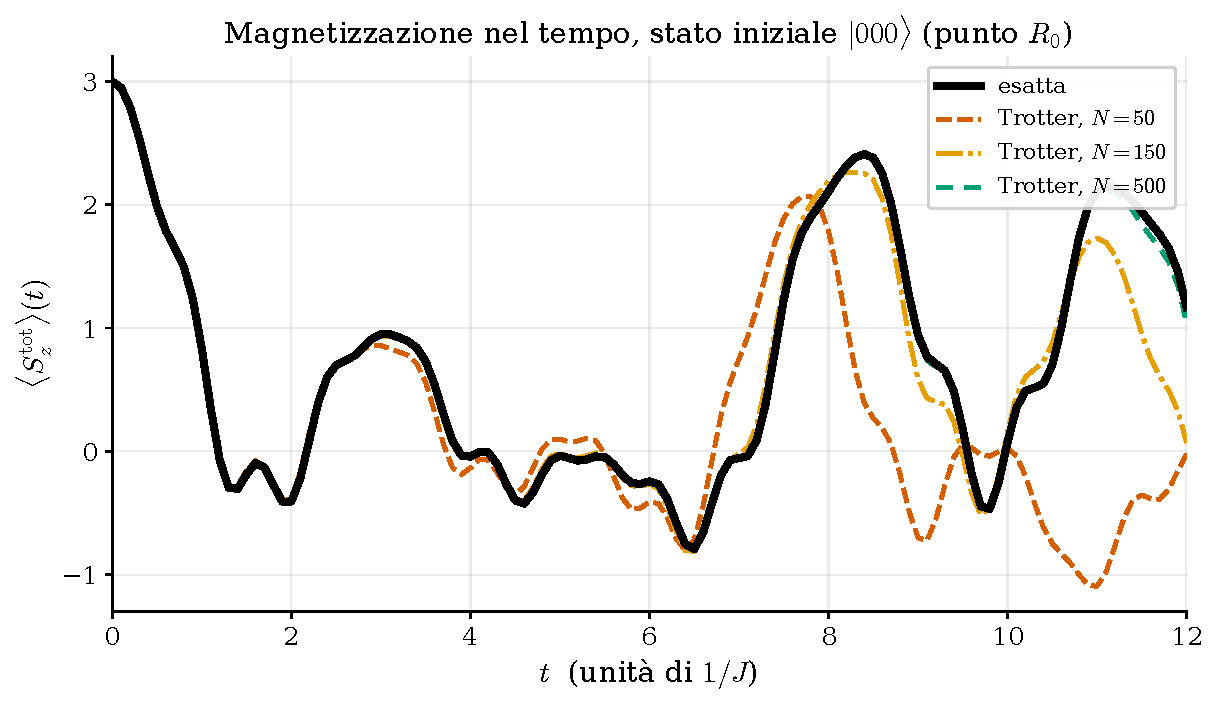
\includegraphics[width=0.86\textwidth]{figure/fig05_trotter_sz_anello}
\caption{$\langle S_z^{\rm tot}\rangle(t)$, stato iniziale $\ket{000}$, punto
$R_0$ ($b/J=0.05$, $D/J=1.93$, dichiarato provvisorio). La curva nera è
l'evoluzione esatta; le altre, Trotter a $N=50,150,500$. Dinamica
volutamente non monocromatica --- un'unica frequenza renderebbe l'errore di
Trotter invisibile.}
\label{fig:sz}
\end{figure}
\FloatBarrier

\verifica{Circuito Qiskit contro matrice compatta (stesso operatore,
elevato a potenza): scarto massimo sulle ampiezze complesse
$4.25\times10^{-15}$ a $t=6$, $N=60$ --- precisione macchina, come atteso
da un confronto fra due modi di calcolare la stessa quantità, non fra due
derivazioni indipendenti. Verificato comunque un dettaglio non banale: la
matrice compatta rispetta il Trotter interno sui tre legami (livelli 1 e
2) e non è l'esponenziale diretto di $H_0$ da solo --- altrimenti il
confronto sarebbe fra due oggetti fisicamente diversi, non fra due modi di
calcolare lo stesso operatore.}

\section{L'errore, e quanto è più lento a convergere rispetto al dimero}

\begin{figure}[htbp]
\centering
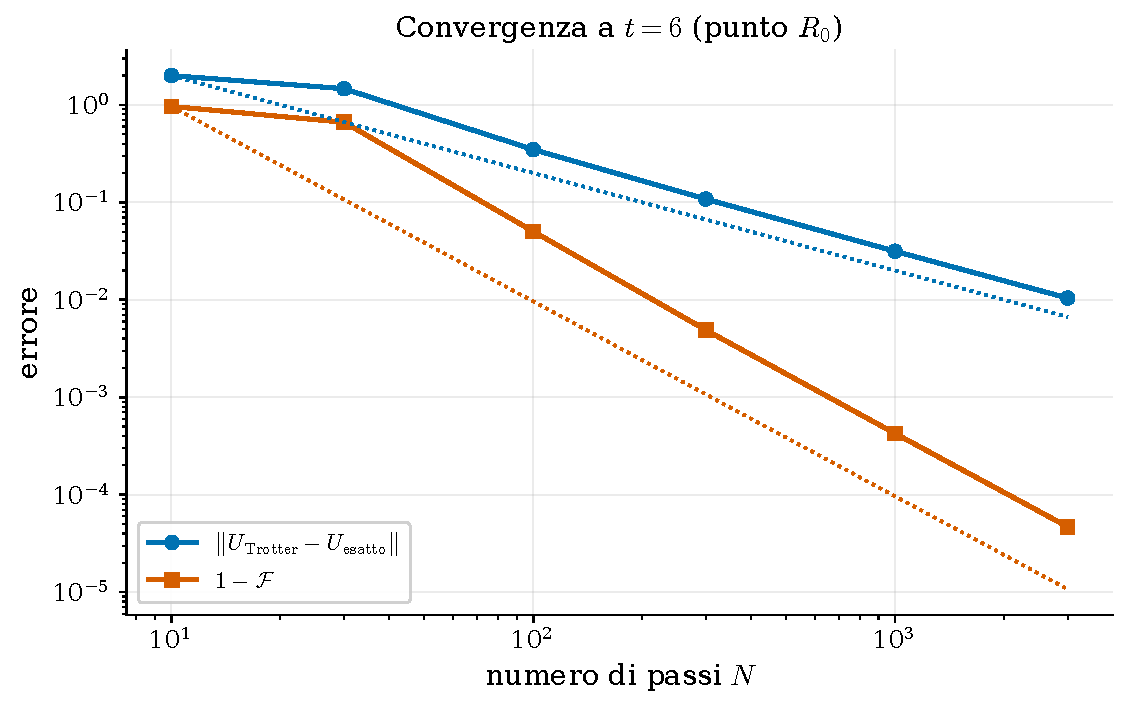
\includegraphics[width=0.74\textwidth]{figure/fig06_trotter_errore_anello}
\caption{Errore a $t=6$ (punto $R_0$), scala doppio-logaritmica. Le rette
punteggiate sono le pendenze asintotiche attese ($-1$ per la norma
dell'operatore, $-2$ per $1-\mathcal F$); gli scostamenti a $N$ piccolo sono
i termini di ordine superiore.}
\label{fig:errore}
\end{figure}
\FloatBarrier

\begin{table}[htbp]
\centering
\small
\renewcommand{\arraystretch}{1.25}
\begin{tabular}{@{}rccc@{}}
\toprule
\rowcolor{grigetto}
$N$ & $\lVert U_{\rm Trotter}-U_{\rm esatto}\rVert$ & $1-\mathcal F$ & soglia raggiunta \\
\midrule
100  & $3.49\times10^{-1}$ & $5.03\times10^{-2}$ & --- \\
300  & $1.08\times10^{-1}$ & $4.90\times10^{-3}$ & $1-\mathcal F<10^{-2}$ \\
1000 & $3.15\times10^{-2}$ & $4.25\times10^{-4}$ & $1-\mathcal F<10^{-3}$ \\
3000 & $1.04\times10^{-2}$ & $4.68\times10^{-5}$ & $1-\mathcal F<10^{-4}$ \\
\bottomrule
\end{tabular}
\caption{Errore a $t=6$, punto $R_0$. Pendenze misurate: $-0.97$ (norma
dell'operatore) e $-1.85$ ($1-\mathcal F$), vicine ai valori teorici $-1,-2$
ma non ancora asintotiche a questi $N$ --- il regime pienamente asintotico
richiede $N$ sensibilmente più grande che sul dimero (dove $N=80$ bastava
per $1-\mathcal F\sim10^{-5}$): qui servono centinaia-migliaia di passi per
soglie comparabili, conseguenza dei due livelli di Trotter interno
aggiuntivi e di un rapporto $D/J\approx1.9$ non piccolo al punto $R_0$.}
\label{tab:errore}
\end{table}
\FloatBarrier

\messaggio{Il dimero converge in decine di passi; il trimero, allo stesso
livello di accuratezza, ne richiede centinaia o migliaia. Non è un
peggioramento generico dovuto alla dimensione del sistema: è dovuto
specificamente al Trotter interno sui legami condivisi (livelli 1 e 2), che
il dimero --- un solo legame --- non ha mai dovuto pagare.}

\section{Quanto costa: il conteggio dei gate}

\begin{table}[htbp]
\centering
\small
\renewcommand{\arraystretch}{1.3}
\begin{tabular}{@{}lcc@{}}
\toprule
\rowcolor{grigetto}
\textbf{Compilazione} & \textbf{CNOT per passo} & \textbf{profondità} \\
\midrule
traduzione diretta, nessuna ottimizzazione & $30$ & $109$ \\
compilazione ottimizzata & $\mathbf{15}$ & $52$ \\
\bottomrule
\end{tabular}
\caption{Costo di un passo esterno di Trotter (tre legami, scambio più DM),
dopo transpilazione in base $\{rz,sx,x,cx\}$. Chiedere al compilatore di
minimizzare dimezza il conteggio di CNOT --- meno drastico del fattore
$>3\times$ osservato sul dimero (dove il passo ha un solo legame, più
margine di fusione), ma comunque un fattore $2\times$ non trascurabile.}
\end{table}
\FloatBarrier

\messaggio{Stessa tensione del dimero fra errore di Trotter (scende con
$N$) ed errore hardware (sale con $N$, $15$ CNOT in più per ogni passo) ---
qui però il costo di raggiungere una data accuratezza di Trotter è molto
più alto (centinaia di passi, non decine), quindi il compromesso fra i due
errori sarà spostato: è il punto centrale del pacchetto sul sistema come
sistema aperto, che riprende esattamente questo conteggio.}

\section{Nota sul punto di lavoro}

Il punto $R_0$ ($b/J=0.05$, $D/J=1.93$) è \textbf{dichiarato provvisorio}:
scelto da uno scan qualitativo per dare una dinamica non monocromatica a
partire da $\ket{000}$, non ancora derivato in modo principiato (a
differenza, per esempio, del punto Scenario A del Documento 2, fissato dal
campo critico esatto). Un pacchetto parallelo di questa stessa serie ha
verificato che $R_0$ è anche, incidentalmente, un punto dove il VQE (ansatz
$W$-2q.6) converge a $\mathcal F>0.999999999$ --- ma questa preparazione VQE
non è usata qui: questo documento, come la dimostrazione originale, parte
sempre da $\ket{000}$, senza preparazione.

\bigskip
\noindent\footnotesize\textit{Riferimento.} Per la decomposizione di
Suzuki--Trotter e la sua analisi dell'errore: N.~Hatano, M.~Suzuki,
\emph{Finding Exponential Product Formulas of Higher Orders}, in
\emph{Quantum Annealing and Other Optimization Methods}, Lecture Notes in
Physics \textbf{679}, Springer (2005).

\end{document}
